\section{Eval plan}

Things I want to show in the eval:

\begin{itemize}
\item That it works for some simple test cases.  This'll include a
  reasonable amount of discussion about what it actually does.
  This'll include showing that the generated fixes work, and some bits
  about their relative performance.  I'd also like to discuss
  whole-program vs. core dump vs. DRS mode here.  This will also
  include a comparison to my implementation of DataCollider.

  Things to show:

  \begin{itemize}
  \item That simple bugs reproduce much more quickly with an enforce
    than without.  It'd also be nice to show that they reproduce more
    quickly under SLI than under DataCollider.
  \item That the analysis to produce them is nice and cheap.
  \item That the performance overhead of the enforcer when the bug
    doesn't reproduce isn't so massive that it'll make bugs less
    likely to reproduce.
  \item That the side-condition checking stuff is both necessary and
    effective.
  \item That we can generate ``reasonable-looking'' fixes for all of
    the test bugs.
  \item That the fixes generated actually fix the intended bug.
  \item That the fixes generated have vaguely plausible performance
    overhead.
  \end{itemize}

  It'd also be quite nice if I could show that the summaries are
  useful for a human trying to fix the bug, but that's likely to be a
  rather hard argument to make.

\item Show that it works for some slightly more realistic artificial
  bugs, probably from ripping sync blocks out of STAMP.
  i.e. real-size programs with artificial bugs.  I currently have one
  bug produced by removing synchronisation from one of the STAMP
  benchmarks for which this works reasonably well; should try to
  expand that a bit.

\item That it could feasibly scale up to something of realistic size.
  Obvious approach here is just to show that we can run the full
  analysis on mysql, apache, thunderbird, and pbzip2.  It's currently
  looking like this will find at most one or two new bugs, which makes
  it all a bit less convincing.  This'll be mostly just showing that
  the analysis does actually complete in a sensible amount of time.
\item I'm going to pick one of those big programs (probably mysql,
  since that's where I've done the most testing so far) and do a few
  more experiments on it:

  \begin{itemize}
  \item Display a CDF of how long it takes to analyse each instruction.
  \item Try turning the various machine simplification passes on and
    off and see what effect that has on the CDF.  Likewise the
    induction rule.
  \item Just directly look at how long the various phases take.
  \item Alias analysis: try turning off the static analysis bit and
    see how much effect that has.
  \item Maybe say something about the number of states in
    {\StateMachines}, how long the symbolic execution takes, etc?
  \end{itemize}

  Aim here is less proving some hypothesis and more just giving a
  decent feeling for where the main costs are.
\item Something about the effects of compiler optimisations?  Probably
  just a couple of paragraphs comparing optimised mysql to debug
  mysql.  Explain why compiler optimisations make some things easier
  and some things harder.
\item I need to show that the dynamic analysis is reasonable.  Ideally
  that'd be by using a static analysis to get an upper bound and then
  showing that they're reasonably close, but implementing that'd be a
  pain in the backside.  Alternative is just to look at convergence
  rates.  I should also look at how large the resulting alias tables
  are for different 
\item I need to show that the tool is actually correctly implemented
  itself.  The small number of bugs found in real programs means that
  this has more than a little bit of a negative-results flavour, so
  this isn't completely trivial.
\end{itemize}

Other things I can look at and evaluate:

\begin{itemize}
\item
  Look at different strategies for combining machines into
  combi-enforcers.
\item
  Look at effect of different analysis window sizes: how many bugs do
  we find, how many false positives, how much time does the analysis
  take.
\item
  Look at how many bugs are killed off by the different clauses of the
  crash definition.
\item
  Investigate performance hit of the enforcement mode, and how that
  depends on the mechanism used to generate the enforcers
  i.e. compiler versus interpreter.
\item
  How much does the W isolation property actually buy us, in terms of
  analysis cost?  How much does it cost us, in terms of lost bugs?
\item
  How large are the CFGs and \StateMachines which we actually
  generate?  Also, how large are the intermediate machines generated
  when we're generating verification conditions?
\item
  Do we actually win anything from using the slightly odd form of SSA?
  Not really sure how to evaluate that; it's sufficiently baked in now
  that I couldn't reasonably replace it to do a cross-eval.
\item
  We handle multi-rooted CFGs completely differently between read and
  write modes.  Does that win/lose anything?
\item
  There are a bunch of places where we have to decide between using
  the simplifier and the sat checker.  Eval which works better for
  each of them.  Downside of evalling this is that it means
  *explaining* the difference between the simplifier and the sat
  checker, which I'd really rather avoid if I can get away with it.
\item
  Crash enforcement: timeout strategies.
\item
  Crash enforcement: how useful is side-condition checking?
\item
  Crash enforcement: how often do we redundantly evaluate side conditions?
\item
  Crash enforcement: Is await-bound-exit actually useful?
  We know it is in silly little artificial test cases, but perhaps not in real programs?
\item
  Currently artificially limit number of live assertions to 5.
  Investigate what effect that has.
\item
  Want something which can evaluate the effectiveness of the
  cross-function alias analysis pass.
\item
  Want something which can evaluate the effectiveness of the phi
  elimination pass.
\item
  Want something which can evaluate the effectiveness of the state
  unification optimisation.
\item
  In order to make the theory behind the crash enforcers work you
  always have to wait for a fixed amount of time when doing unbound
  message operations, even if someone arrives before the time has
  passed.  Most of the time, that extra delay is wasted.  Look at how
  much time is wasted, and how bad it would be to just not do that.
\end{itemize}

\section{Artificial bugs}

I now present the results of running {\implementation} on a number of
artificial bugs, showing that it assists in both reproducing the bugs
and fixing them, along with some discussion of what the various
analysis phases actually do.

Lookup between bug numbers and names:

\begin{itemize}
\item 1 -- Simple TOCTOU
\item 2 -- Indexed TOCTOU
\item 3 -- Indexed TOCTOU with rare writes
\item 4 -- Indexed TOCTOU with rare reads
\item 5 -- Multi-variable consistency constraint
\item 6 -- Context-dependent TOCTOU; multiple calls to \verb|f|, but
  only one has the bug of interest.
\item 7 -- Cross-function TOCTOU; check in one function, use in the
  function it returns to.
\item 8 -- Write to read hazard on the read side races with a wild
  store.
\item 9 -- Multiple possible bugs in one program, requiring combined
  enforcement plans.
\item 10 -- Lots of threads on the read side.
\item 11 -- Something which couldn't be found by Chess or
  DataCollider.  That really means something with at least three
  mandatory preemptions.
\item 12 -- Something which demonstrates data-dependent happens-before
  graphs.
\item 13 -- A false positive -- something where the main analysis
  thinks there might be a bug, but there isn't, and so the enforcer
  can't enforce it.
\item 14 -- Something which nicely illustrates the cross-function
  alias analysis stuff.  Tricky part of this is that programs need to
  be fairly complex before this kicks in.
\item 15 -- Something which illustrates the importance of the Phi
  elimination pass.  Likewise.
\end{itemize}

\subsubsection{Simple time-of-check, time-of-use (TOCTOU) bug (simple\_toctou)}
\label{sect:eval:art:simple_toctou}

\todo{The discussion here is painfully detailed.  I think that's
  reasonable for the first bug discussed, but later ones are going to
  have to be much more high-level.  To be honest, I'm not entirely
  convinced that this bit is all that interesting, but I think I
  should probably copy-and-paste the complete tool output into the
  dissertation at least once, just to prove that it exists.}

\todo{Perhaps I should move some of this discussion a bit earlier and
  treat it as an example?}

\begin{figure}
  \begin{subfloat}
    \begin{minipage}{50mm}
\begin{verbatim}
while (1) {
   STOP_ANALYSIS();
   if (global_ptr != NULL)
       *global_ptr = 5;
   STOP_ANALYSIS();
}
\end{verbatim}
    \end{minipage}
    \caption{Read-side}
  \end{subfloat}
  \begin{subfloat}
    \begin{minipage}{50mm}
\begin{verbatim}
while (1) {
    global_ptr = &t;
    sleep(1 second);

    STOP_ANALYSIS();
    global_ptr = NULL;
    STOP_ANALYSIS();
}
\end{verbatim}
    \end{minipage}
    \caption{Write-side}
  \end{subfloat}
  \label{fig:eval:simple_toctou}
  \caption{The two sides of the simple\_toctou bug.}
\end{figure}

\begin{figure}
  \begin{subfloat}
    \begin{minipage}{70mm}
\begin{verbatim}
  400624: mov    (global_ptr),%rax
  40062b: test   %rax,%rax
  40062e: je     40063d
  400630: mov    (global_ptr),%rax
  400637: movl   $0x5,(%rax)
  40063d:
\end{verbatim}
    \end{minipage}
    \caption{Read side}
  \end{subfloat}
  \begin{subfloat}
    \begin{minipage}{70mm}
\begin{verbatim}
  400815: movq   $0x0,(global_ptr)
  400820:
\end{verbatim}
    \end{minipage}
    \caption{Write side}
  \end{subfloat}
  \label{fig:eval:simple_toctou_compiled}
  \caption{Disassembly of the program in figure~\ref{fig:eval:simple_toctou}.}
\end{figure}

This is the simplest possible kind of concurrency bug: as
single-variable time-of-check, time-of-use race.  The two threads
involved are shown in figure~\ref{fig:eval:simple_toctou}.  The intent
here is to model a very simple structure which is accessed frequently
but updated rarely.  The bug is, of course, that the updating thread
might set \verb|global_ptr| to \verb|NULL| in between the two reads of
it in the reading thread, causing the reading thread to crash when it
dereferences the pointer it loaded.  \verb|STOP_ANALYSIS()| is a
marker which prevents {\technique}'s analysis from exploring past that
point when build the CFGs from which {\StateMachines} are constructed.
It is used here to help keep the crash summaries generated simple and
easily explained; {\implementation} is able to reproduce and fix the
bug even without those markers\editorial{Could last time I tried it,
  probably worth checking that again with the current version.}.
Compiling this program produced the machine code fragments illustrated
in figure~\ref{fig:eval:simple_toctou_compiled}.

\begin{figure}
  \begin{minipage}{100mm}
\begin{verbatim}
Load Machine:
CFG:
-1-------->cfg6: {0x400624} -> cfg5:branch
.          cfg5: {0x40062b} -> cfg4:branch
.          cfg4: {0x40062e} -> cfg3:default
.          cfg3: {0x400630}
l1: {{0x400624}:LOAD tmp1:1:1:I64 <- *(0x601040:I64):normal@mai1:1 then l2}
l2: {0x40062e}: if ((0x0:I64 == GET:I64(tmp1:1:1))) then l3 else l4
l3: <survive>
l4: {{0x400630}:LOAD tmp1:1:2:I64 <- *(0x601040:I64):normal@mai1:2 then l5}
l5: {0x400637}: if (BadPtr(GET:I64(tmp1:1:2))) then l8 else l3
l8: <crash>
Root: l1
Store Machine:
CFG:
-98------->cfg52: {0x400815}
l7: {{0x400815}:*(0x601040:I64):normal <- 0x0:I64 @ mai98:4 then l8}
l8: <crash>
Root: l7
Memory access identifiers:
        mai1:1 -> {cfg6}
        mai1:2 -> {cfg3}
        mai98:4 -> {cfg52}
Aliasing:
        mai1:1 <-> mai98:4
        mai1:2 <-> mai98:4
Verification condition: (!((mai1:2 <-< mai98:4)) && (mai1:1 <-< mai98:4))
\end{verbatim}
  \end{minipage}
  \caption{Crash summary generated for the program in
    figure~\ref{fig:eval:simple_toctou}.}
  \label{fig:eval:simple_toctou_summary}
\end{figure}

\begin{figure}
  \begin{tikzpicture}
    \node[draw] (l1) {400624};
    \node[draw, below right = of l1] (l2) {400815};
    \node[draw, below left = of l2] (l3) {40063e};
    \draw[->] (l1) -- (l3);
    \draw[->, happensBeforeEdge] (l1) -- (l2);
    \draw[->, happensBeforeEdge] (l2) -- (l3);
  \end{tikzpicture}
  \caption{Happens-before graph to be enforced for simple\_toctou}
  \label{fig:eval:simple_toctou_hb_graph}
\end{figure}

SLI produces a single candidate bug for this program, shown in
figure~\ref{fig:eval:simple_toctou_summary}.  This is hopefully
reasonably easy to understand at this point.  The candidate bug
consists of several parts:

\begin{itemize}
\item The {\StateMachines} for the read and write sides of the race.
  In this case, the load machine has been assigned thread identifier 1
  and the store machine has been assigned thread identifier 98.  These
  identifiers are completely arbitrary.
\item Control flow graph fragments for the two sides.  The read side
  here contains CFG nodes three through 6, while the store machine has
  CFG node 52; these identifiers are arbitrary.  In this case the CFGs
  are largely uninteresting, but in a more complex example these
  fragments would include details of which nodes were created by loop
  unrolling and some information on the function call structure of the
  program.

  Note that the instruction which actually crashes, \verb|400637| is
  not included in the CFGs.  This is because it is completely
  irrelevant to the behaviour which is actually being investigated: by
  the time that instruction executes, the program has either avoided
  the purported bug or is doomed to crash, and so it cannot tell us
  anything useful about the nature of the bug.

  Note also that the read-side CFG does not include the control-flow
  edge from \verb|40062e| to \verb|40063d|.  If the program follows
  that edge then the bug will definitely be avoided, as the crashing
  instruction will not run, and so it is perfectly appropriate to
  exclude it from the CFG here.
\item A memory access identifier table, showing how memory access
  identifiers map into CFG nodes, or, in other words, how the accesses
  analysed by SLI's main analysis passes correspond to accesses made
  by the program itself.  In this case, that mapping is trivial, and
  each memory access identifier corresponds to a single CFG node.  In
  in a more complex example SLI might merge several similar program
  accesses into a single \StateMachine-level accesses, and in that
  case a single memory access identifier might map to multiple CFG
  nodes.
\item An aliasing table, showing which memory accesses might
  potentially access the same memory, according to the
  dynamically-collected aliasing table.
\item The verification condition.  This is the condition which must
  hold for the bug being investigated to reproduce when the two
  \StateMachines are run in parallel.  In this case, it consists of
  just two happens-before edges, \verb|mai1:1 <-< mai98:4| and
  \verb|!((mai1:2 <-< mai98:4))|, which between them indicate that the
  bug will reproduce precisely when memory access 4 in thread 98
  intervenes between memory accesses 1 and 2 in thread 1.  In other
  words, the program will crash when the store thread sets
  \verb|global_ptr| to \verb|NULL| in between the two loads of
  \verb|global_ptr| in the load thread, precisely as desired.
\end{itemize}

\begin{figure}
  \begin{minipage}{100mm}
\begin{verbatim}
Crash enforcement plan:
        Threads: T1:1 = {t1}; T1:98 = {t2}
        Roots: t1 = {cfg6}; t2 = {cfg52}
        CFG:
                cfg3:t1: successors = {}
                cfg4:t1: successors = {cfg3}
                cfg5:t1: successors = {cfg4}
                cfg6:t1: successors = {cfg5}
                cfg52:t2: successors = {}
        Label to RIP table:
                1:cfg3 -> {0x400630}
                1:cfg4 -> {0x40062e}
                1:cfg5 -> {0x40062b}
                1:cfg6 -> {0x400624}
                1:cfg52 -> {0x400815}
        Happens before map:
                cfg3:t1 -> {43708: cfg52:t2 <-< cfg3:t1}
                cfg6:t1 -> {43707: cfg6:t1 <-< cfg52:t2}
                cfg52:t2 -> {43707: cfg6:t1 <-< cfg52:t2,
                             43708: cfg52:t2 <-< cfg3:t1}
Patch = {0x400624, 0x400815}, Cont = {}
\end{verbatim}
  \end{minipage}
  \caption{Crash enforcement plan generated for the simple\_toctou
    bug} \todo{Having said I wanted to copy and paste the output,
    that's a slightly simplified version.  Should probably fix the
    pretty printer so that I can just copy and paste it.}
  \label{fig:eval:simple_toctou_cep}
\end{figure}

The next step of the pipeline is to take that crash summary and
convert it into a crash enforcement plan, shown in
figure~\ref{fig:eval:simple_toctou_cep}.  In this case, no side
conditions need to be checked and no program-level values need to be
stashed, and so this is a direct encoding of the verification
condition and control flow graph from
figure~\ref{fig:eval:simple_toctou_summary}.  There is only one bug to
be enforced and that bug only reproduces in a single possible
happens-before graph and so there is precisely one plan-level thread
for every summary-level one.  Finally, the patch strategy generated is
very simple, with a single $Patch$ entry for the first instruction in
each CFG fragment and no $Cont$ entries, because the test program's
control flow is such that that will not risk the
branch-to-corrupted-instruction problem.

\todo{Hmm.  A lot of the features of the plan only really make sense
  when you're combining multiple candidate bugs into a single
  enforcement plan, which means they're hard to describe in this
  single-candidate example.}

\todo{I should come up with a less ugly way of displaying the damn
  things.}

The plan can then be loaded into the buggy program in order to make
the bug reproduce more easily.  In this particular case the results
are somewhat unimpressive, as this bug already reproduces quite
easily, but still show a small improvement in reproduction time.

The time to reproduce a bug of this kind follows a roughly exponential
distribution, as each iteration of the write loop has a roughly
independent chance of causing the read loop to crash.  I ran each
configuration (with enforcer, without enforcer) ten times on an
otherwise idle machine and timed how long it took for them to crash.
As might be expected, the version without the enforcer always took a
roughly whole number of seconds to crash, as the write side runs after
a whole number of seconds has passed.  The mean time before the
program crashed was 5.2 seconds, so each iteration of the write side
has a roughly 20\% chance of causing the read side to
crash\editorial{Need to re-do that stat with more data}.

\begin{figure}
  \tikzset{label/.style = {anchor=north west}}
  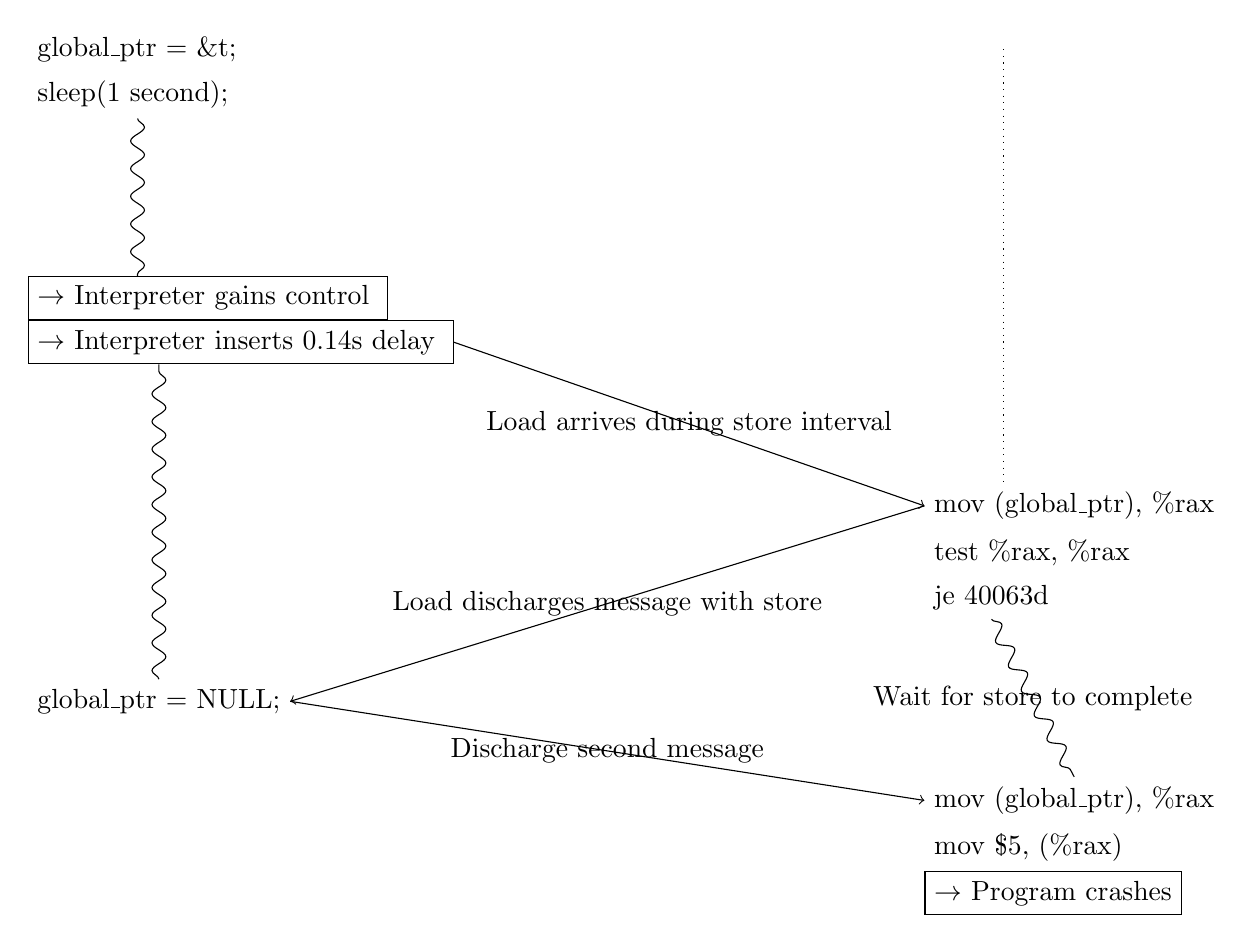
\begin{tikzpicture}[node distance = 0 and 0]
    \begin{scope}[align=left]
      \node[] (storeSt1) at (0,2) {global\_ptr = {\&}t;};
      \node[label] at (storeSt1.south west) (storeSleep) { sleep(1 second); };
      \path (storeSleep.south west) -- +(0,-2cm) node [name=storeTrap, label, draw] { $\rightarrow$ Interpreter gains control };
      \draw[decorate,decoration={snake}] (storeSleep.south) -- +(0,-2cm);
      \node[draw, label] at (storeTrap.south west) (storeDelay) { $\rightarrow$ Interpreter inserts 0.14s delay };
      \path (storeDelay.south west) -- +(0,-4cm) node [name=storeSt2, label] { global\_ptr = NULL;};
      \draw[decorate,decoration={snake}] (storeSt2.north) -- +(0,4cm);
    \end{scope}

    \begin{scope}[xshift=10cm]
      \node[label] at (0,-3.5cm) (loadLdA2) {mov (global\_ptr), \%rax };
      \draw[dotted] (1,2) -- +(0,-5.5cm);
      \node[label] at (loadLdA2.south west) (loadTest2) {test \%rax, \%rax };
      \node[label] at (loadTest2.south west) (loadJe2) {je 40063d};
      \path (loadJe2.south west) -- +(0,-2cm) node [name=loadLdB,label] { mov (global\_ptr), \%rax};
      \draw[decorate,decoration={snake}] (loadJe2.south) to node {Wait for store to complete} (loadLdB.north);
      \node[label] at (loadLdB.south west) (loadSt) {mov \$5, (\%rax)};
      \node[label,draw] at (loadSt.south west) {$\rightarrow$ Program crashes};
    \end{scope}

    \draw[->] (storeDelay.east) to node {Load arrives during store interval} (loadLdA2.west);
    \draw[->] (loadLdA2.west) to node {Load discharges message with store} (storeSt2.east);
    \draw[->] (storeSt2.east) to node {Discharge second message} (loadLdB.west);
  \end{tikzpicture}
  \caption{Enforcing the simple\_toctou bug.  Dotted lines indicate
    the program thread running some uninteresting code, wavey lines
    indicate the program thread sleeping.  The program crashes after
    roughly 1.14 seconds.}
\end{figure}

With the enforcer loaded and delays set to be between 100ms and 200ms,
the program crashes after between 1.1 and 1.2 seconds, with a uniform
distribution between the two.  This delay consists of two components:

\begin{itemize}
\item One second, which is caused by the call to \verb|sleep| in the
  test harness.
\item An additional 100 to 200ms, which is caused by the RX message
  delay.  The write thread starts its critical section at one second
  in and must immediately wait for a read thread to arrive.  In this
  configuration, the thread will wait for between 100 and 200
  milliseconds.
\end{itemize}

To confirm this explanation, I modified the interpreter to seed the
random number generator with a constant, with the result that the
first delay was fixed at 144ms.  In this configuration, the program
crashed after $1.144 \pm 0.002$ seconds (mean and standard deviation
of ten runs), roughly as expected.  Note that this distribution was
not Gaussian, due to the presence of positive outliers, but that the
largest of these, 1.153 seconds, was not large enough to meaningfully
change the conclusions.

\textbf{Statistical considerations} As noted above, without the
enforcer the program usually crashes after a little over five seconds
while with the enforcer applied it crashes after between 1.1 and 1.2
seconds.  It would be useful to have some indication of the
uncertainty in the former number.  Characterising the time taken
without an enforcer is, however, somewhat problematic, as the
distribution of times taken is leptokurtic: the mean and standard
deviation here was $5.0 \pm 5.1$\editorial{only ten runs; redo
  stats}, even though the time taken is always positive, indicating
that the standard deviation is pretty much meaningless.  As such, the
distribution must be characterised in some other way.  From
theoretical arguments, I expected the distribution to be a
geometrically distributed integer multiplied by roughly one second,
and so one obvious approach would be to characterise it by the $p$
value of the geometric distribution, obtained using the method of
moments.  I used a resampling method to obtain the uncertainty of this
value: I ran the test 10,000 times, used that data to generate 10,000
random samples selections of 100 samples, with replacement, and then
re-estimated the $p$ value for each of those samples.  The resulting
distribution had a mean of $0.20$ and a population standard deviation
of $0.02$.  It passed both the Anderson-Darling and Jarque-Bera
normality tests at the 90\% level, and so I am reasonably confident
that this is a reasonable characterisation of that distribution.
\todo{Actually, that resampling was only done from a pool of 300 runs,
  so I need to re-do it with a bit more data.}

\todo{This is a bit unnecessary, in the sense that nobody else ever
  bothers, but also completely necessary, in the sense that without
  that the numbers simply don't mean anything.}

\todo{I should really do a goodness of fit test to make sure that the
  distribution really is geometric there.}

The fix generated in this case is very simple and contains two
critical sections, one covering \verb|400624| to \verb|400630| and the
other covering the single instruction \verb|400815|.  Notice that, as
in the enforcer, the instruction which crashes, \verb|400637|, is
\emph{not} included in any critical section.  The patch itself is, in
this case, rather large relative to the original program code (179
bytes rather than 26).  This is mostly because the machine code to be
protected is itself quite small and so the function call sequence used
to acquire or release the patch lock completely dominates the total
size of the patch.

\textbf{Performance} It is not completely straightforwards to
characterise the performance of this program without the enforcer
applied as it very rarely runs long enough for to obtain a meaningful
number.  The approach I have taken is to run the test program
repeatedly until it managed to survive for ten seconds and then treat
the number of iterations of the read thread in those ten seconds as
the performance metric.  This average value of the metric was
$351*10^6 \pm 4*10^6$ but this was not Gaussian, failing the
Anderson-Darling test at the 99.5\% level.  Excluding the two lowest
values as outliers gave a result of $352.5 * 10^6 \pm 0.1 * 10^6$ and
those results passed both the Anderson-Darling and Jarque-Bera
normality tests at 90\%.

With the fix applied, performance in a full ten-element run dropped to
$95.4 * 10^6 \pm 0.3 * 10^6$ with no outliers, and this distribution
passed both normality tests at the 90\% level.  This gives an overhead
of roughly a factor of 3.7.  This is obviously rather large, but is
probably close to {\technique}'s worst case: the read-side critical
section is very small and runs with very high frequency, and so the
patch must acquire and release the lock with similarly high frequency
and these lock operations dominate the time taken.  Any realistic test
would usually have much lower overhead, assuming lock contention does
not become a factor.  Even in this case, a factor of four overhead is
not completely unreasonable when the alternative is a program which
crashes frequently.

\todo{I should probably re-run those experiments now that I've decided
  on a statistical protocol.}

\todo{Give details of the machine the test is running on.}

\todo{Give some breakdown of where the overhead comes from.  I
  strongly suspect that it's almost all down to the cost of acquiring
  and releasing the lock; it'd be nice to confirm that.}

\todo{Time taken to do analysis?}

\subsubsection{Indexed TOCTOU bug (indexed\_toctou)}

\todo{I don't currently seed the random number generator inside the
  test program.  Not sure what effect that'll have on all those
  stats.}

In this variant of a TOCTOU bug, there are multiple instances of the
structure which is being raced on and the bug will only manifest if
the reading and writing threads happen to coincide.  This bug
exercises the side-condition-checking part of SLI.  The code involved
in the race is shown in figure~\ref{fig:eval:indexed_toctou}.  Except
where otherwise noted, \verb|NR_PTRS| is set to 100.

\begin{figure}
  \begin{subfloat}
    \begin{minipage}{50mm}
\begin{verbatim}
while (1) {
  idx = random() % NR_PTRS;
  STOP_ANALYSIS();
  if (global_ptrs[idx] != NULL)
    *(global_ptrs[idx]) = 5;
  STOP_ANALYSIS();
}
\end{verbatim}
    \end{minipage}
    \caption{Read side}
  \end{subfloat}
  \begin{subfloat}
    \begin{minipage}{50mm}
\begin{verbatim}
while (1) {
  idx = random() % NR_PTRS;
  STOP_ANALYSIS();
  global_ptrs[idx] = NULL;
  STOP_ANALYSIS();
  global_ptrs[idx] = &t;
}
\end{verbatim}
    \end{minipage}
    \caption{Write side}
  \end{subfloat}
  \caption{The two sides of the indexed\_toctou bug.}
  \label{fig:eval:indexed_toctou}
\end{figure}

The summary, fix, and enforcer produced here are essentially the same
as for indexed\_toctou except for the addition of a side-condition
requiring the two indices to match up, and so is not discussed in
detail here.

With no enforcer loaded, this bug reproduces in $6 \pm 8$ seconds, in
a test with 100 samples, which again strongly suggests it to be
non-Gaussian.  In this case, the distribution appears to be
exponential, and so I characterise it by the $\lambda$ parameter of
the exponential distribution and use a resampling approach to estimate
the variance of that parameter.  Taking one hundred samples of size
one hundred from a pool of 158 results\editorial{Re-do now with more
  data.} gave an estimated $\lambda$ of $0.16 \pm 0.02$, and that
result passes the Anderson-Darling and Jarque-Bera normality tests at
the 90\% level.

\todo{Proper goodness-of-fit test on the exponential distribution?}

With the enforcer loaded, the time taken to reproduce the bug was
roughly uniformly distributed between 100 and 200ms, which is as
expected if the enforcer is able to trigger the crash after a single
delay. \todo{Again, goodness of fit test on that uniform dist.}

I also investigated the behaviour of this test with an enforcer loaded
but no side condition checking performed.  In that case, the bug
reproduced after $1.72 \pm 2.81$ seconds (mean and standard deviation
of one hundred runs).  Resampling and fitting an exponential
distribution gave a $lambda$ parameter here of $0.62 \pm 0.06$, and so
the enforcer without side condition checking produces does cause the
bug to be reproduced significantly more often than simply running the
program without side-condition checking, but not nearly as quickly
as with the checking.

As a further test, I investigated what happens when the length of the
delays is modified, first by reducing it to between 10 and 20
milliseconds and then by increasing it to between 1000 and 2000
milliseconds.  The results are shown in
table~\ref{table:eval:indexedtoctou:delay}.  The important point to
note here is that disabling side-condition checking and setting a
timeout of one second actually leads to a lower bug reproduction rate
than simply running without an enforcer of any sort, and increasing
the delay further would exacerbate this problem.  Of course, one to
two seconds is a rather long time to wait in order to reproduce a
race, but this might still be appropriate if the bug to be
investigated is in code which is executed very infrequently.

\begin{table}
\begin{tabular}{lll}
Delay range  & With side-condition checking          & Without side-condition checking \\
10-20ms      & $\lambda = 58 \pm 0.7/s$              & $\lambda = 5.3 \pm 1.97/s$ \\
100-200ms    & $t = 100 - 200ms$                     & $\lambda = 1.72 \pm 2.81/s$ \\
1000-2000ms  & $t = 1000 - 2000ms$                   & $\lambda = 0.13 \pm 0.001/s$ \\
\end{tabular}
\caption{Effect of side condition and delay parameter on time taken to
  reproduce the indexed\_toctou bug.}  \todo{Some of those are quite
  small sample sizes; redo.}
\label{table:eval:indexedtoctou:delay}
\end{table}

As a final test, I investigated the effect changing the \verb|NR_PTRS|
parameter, and how that interacted with the delay parameter.  The
results are shown in table~\ref{table:eval:indexedtoctou:nrptrs}.

\todo{The NR\_PTRS = 1000 configuration with no side conditions
  definitely isn't Gaussian, but I don't have enough data to say more
  than that.  Also, for the full enforcer, the NR\_PTRS = 1000 is now
  5--95\% interval, rather than full interval, because we're starting
  to get enough noise that that makes more sense.}

\todo{Not sure why the no-enforcer results aren't monotonic.}

\begin{table}
\begin{tabular}{llll}
NR\_PTRS & Full enforcer             & No side conditions          & No enforcer               \\
10       & $\lambda = 6.4 \pm 0.2/s$ & $\lambda = 1.27 \pm 0.02/s$ & $\lambda = 0.32 \pm 0.05$ \\
100      & $t = 100 - 200ms$         & $\lambda = 0.62 \pm 0.06/s$ & $\lambda = 0.16 \pm 0.02$ \\
1000     & $t = 110 - 201ms$         & $t = 33.1 \pm 8.8$          & $\lambda = 0.24 \pm 0.02$ \\
\end{tabular}
\caption{Time taken to reproduce indexed\_toctou as NR\_PTRs changes.}
\todo{Stats slightly dubious here, especially the }
\label{table:eval:indexedtoctou:nrptrs}
\end{table}

The automatic fix generator works well with this bug, and produces
roughly the same fix as it did in the simple\_toctou bug: one critical
section which covers the two critical loads in the read thread and one
which covers the critical store in the write thread.  To characterise
the performance overheads of the fix I again counted the number of
times the read and write loops execute per second with and without the
fix applied, running the test for ten seconds and discarding any runs
in which the test program crashed.  Without a fix applied, the test
completed the read loop $9.8 * 10^5 \pm 0.7 * 10^5$ times per second
and the write loop $8.5 \pm 0.5 * 10^5$ times per second; with a fix,
it completed $9.5 * 10^5 \pm 0.6 * 10^5$ read loops and $8.5 * 10^5
\pm 0.4 * 10^5$ write loops (mean and standard deviation of ten runs).
The overhead is therefore not statistically significant in this test.
This is largely because both loops include calls to \verb|random|,
which is rather expensive and completely swamps the cost of the
additional synchronisation.

\todo{I don't believe for a minute that those are Gaussian.}



\subsubsection{Biassed indexed TOCTOU bugs (read\_indexed\_toctou, write\_indexed\_toctou)}

These bugs are essentially similar to the indexed\_toctou, except with
additional delays such that either the write operation (for
write\_indexed\_toctou) or the read operation (for
read\_indexed\_toctou) is far more common than the other.  This test
illustrates the importance of rebalancing delays between the various
happens-before edges in the crash enforcement plans.

\subsubsection{Multi-variable consistency constraint (multi\_variable)}

This bug is intended to illustrate that {\technique} is able to
correctly analyse multi-variable atomicity violations.  The read side
is simply:

\begin{verbatim}
while (1) {
   STOP_ANALYSIS();
   v1 = global1;
   v2 = global2;
   assert(v1 == v2);
   STOP_ANALYSIS();
   usleep(10000);
}
\end{verbatim}

The write side is:

\begin{verbatim}
while (1) {
  usleep(100000);
  STOP_ANALYSIS();
  global1 = 5;
  global2 = 5;
  STOP_ANALYSIS();
  usleep(100000);
  STOP_ANALYSIS();
  global1 = 7;
  global2 = 7;
  STOP_ANALYSIS();
}
\end{verbatim}

Note that this also illustrates {\technique}'s ability to handle
\verb|__assert_fail|-type crashes, in addition to bad pointer
dereference ones.

This bug could not be handled by tools such as Kivati\needCite{}, as
it involves multiple variables, but can be handled by {\technique}:
the bug is reproduced quickly by the enforcer, and a correct and
low-overhead fix is generated automatically.

\subsubsection{Context-dependent races (context)}

This test is similar to simple\_toctou, except that the behaviour
depends on the function's call context.  It is structured like this:

\begin{verbatim}
f(int **ptr) {
    if (*ptr)
        **ptr = 5;   
}
read_thread() {
    while (1) {
        if (random() % 1000 == 0) {
            STOP_ANALYSIS();
            f(&global_ptr1);
            STOP_ANALYSIS();
        } else {
            STOP_ANALYSIS();
            f(&global_ptr2);
            STOP_ANALYSIS();
        }
    }
}        
write_thread() {
    while (1) {
        STOP_ANALYSIS();
        global_ptr1 = &t;
        STOP_ANALYSIS();
        sleep(1ms);
        STOP_ANALYSIS();
        global_ptr1 = NULL;
        STOP_ANALYSIS();
    }
}
\end{verbatim}

Here, there are two calls to \verb|f|, only one of which could ever
possibly exhibit the bug, and that call is much less frequent than the
other one.  Reproducing the bug quickly is therefore only possible if
the crash enforcer checks the calling context before inserting any
large additional delays.

\todo{It'd be worthwhile trying this test again with a STOP\_ANALYSIS
  at the top of f, just to confirm that we correctly generate a
  side-condition on ptr with the same effect as checking context even
  when we don't backtrack far enough to know what the context is.}

\subsubsection{Write-to-read hazard (write\_to\_read)}

This test demonstrates a bug on the edge of what SLI can handle.
Because of the W isolation property in the bug definition, SLI cannot
handle any bugs in which the write thread reads a memory location
which has been written to by the read thread.  It is, however,
supposed to be able to handle the case where the read thread reads a
location which has been written by the read thread, and in particular
the case where a write in the read thread races with a write in the
write thread and the result is then read by the read thread.  This
test demonstrates that case.

(In other words, there is a write-to-read hazard in the read thread
which is potentially interrupted by the write thread.)

The read side is simple:

\begin{verbatim}
global_ptr = &t;
*global_ptr = 5;
\end{verbatim}

The write side is then this:

\begin{verbatim}
global_ptr = NULL;
\end{verbatim}

Both sides run in a tight loop without any delays.  Despite this, it
still often takes several seconds for the bug to reproduce without an
enforcement patch applied, during which time the two critical sections
may run hundreds of millions of times.  A more realistic test would
run the two sections far less frequently, and so might require
hundreds of years of CPU time to reproduce the bug.  The SLI-generated
enforcer patch, by contrast, can reliably reproduce this bug in a few
hundred milliseconds.

\todo{I think it might be interesting to investigate this a bit more.
  I have a sneaking suspicion that it won't reproduce at all if you
  run on bare metal without any interrupts, and that it pretty much
  only reproes if you get a timer interrupt at precisely the right (or
  wrong) place.  Could maybe get a paragraph or so of useful
  discussion out of that if I had some evidence.  Plus, it's the kind
  of experiment which looks impressive but is actually really easy,
  so, you know, win.}

\subsubsection{Multiple bugs (multi\_bugs)}

This test combines simple\_toctou and write\_to\_read into a single
test, and demonstrates SLI's ability to exercise several bugs using a
single enforcer.  This is useful when testing with large programs;
something like mysqld can easily generate thousands of candidate bugs,
and having to test each one individually would become quite tedious,
but testing dozens at a time is far more reasonable.

The read side of the test is structured like this:

\begin{verbatim}
while (1) {
    r = select_test();
    STOP_ANALYSIS();
    if (r)
        simple_toctou();
    else
        write_to_read();
    STOP_ANALYSIS();
}
\end{verbatim}

The behaviour of \verb|select_test| is configurable at run time.  It
can either choose between the tests at random, always select one, or
always select the other.  The write side of the test is structured
like this:

\begin{verbatim}
for (i = 0; i < 2000000; i++) {
    STOP_ANALYSIS();
    write_to_read_write_side();
    STOP_ANALYSIS();
}
STOP_ANALYSIS();
simple_toctou_write_side();
STOP_ANALYSIS();
\end{verbatim}

The constant \verb|2000000| was chosen such that with no enforcer
applied and with the read side configured to choose the two tests with
equal probability the two bugs reproduce with roughly equal frequency.

In this test, SLI correctly generates two candidate bugs (one for each
component bug).  These can either be instantiated into separate
enforcers (which have the expected behaviour of making one bug
reproduce quickly while having no effect on the other) or combined
into a single enforcer.  If the test is configured to always use one
bug or the other then the combined enforcer consistently reproduces
that, as desired.  More surprisingly, if the test is configured to
select a sub-test randomly then the enforcer always reproduces the
write\_to\_read bug, simply because the enforcer reproduces the bug
quickly enough that the write side of the simple\_toctou write side
never runs.

\subsubsection{Multiple read threads (multi\_threads)}

\todo{Write me.}

\subsubsection{Complicated happens-before graphs (complex\_hb)}

This test is intended to illustrate {\technique}'s ability to handle
more complicated happens-before graphs which require more than two
context switches.  This kind of bug defeats some existing tools such
as Chess\needCite{} or DataCollider\needCite{}.  The test is
structured like so:

\begin{verbatim}
while (1) {
   STOP_ANALYSIS();
   x' = x;
   x'' = x;
   x''' = x;
   assert(!((x' == 0) && (x'' == 1) && (x''' == 2) ));
   STOP_ANALYSIS();
}
\end{verbatim}

And the write side is:

\begin{verbatim}
while (1) {
  STOP_ANALYSIS();
  x = 0;
  x = 1;
  x = 2;
  STOP_ANALYSIS();
  delay();
}
\end{verbatim}

\begin{figure}
  \begin{tikzpicture}
    \node[draw] (x0) {x = 0};
    \node[draw, below right = of x0] (xp) {x' = x};
    \node[draw, below left = of xp] (x1) {x = 1};
    \node[draw, below right = of x1] (xpp) {x'' = x};
    \node[draw, below left = of xpp] (x2) {x = 2};
    \node[draw, below right = of x2] (xppp) {x''' = x};
    \draw[->, happensBeforeEdge] (x0) -- (xp);
    \draw[->, happensBeforeEdge] (xp) -- (x1);
    \draw[->, happensBeforeEdge] (x1) -- (xpp);
    \draw[->, happensBeforeEdge] (xpp) -- (x2);
    \draw[->, happensBeforeEdge] (x2) -- (xppp);
    \draw[->] (x0) -- (x1);
    \draw[->] (x1) -- (x2);
    \draw[->] (xp) -- (xpp);
    \draw[->] (xpp) -- (xppp);
  \end{tikzpicture}
  \caption{Happens-before graph necessary to reproduce the complex\_hb
    bug.}
  \label{fig:eval:complex_hb}
\end{figure}

In this case, the bug will only reproduce if the happens-before graph
is as shown in figure~\ref{fig:eval:complex_hb}.  This is a difficult
bug for Chess and DataCollider to handle, for somewhat different
reasons.

For Chess, whether the bug can be correctly handled will depend on how
many context switches the analysis is configured to explore, and any
setting of three or more should be able to trigger it.  The value used
in the Chess paper is two, and so in that configuration this bug would
not be correctly handled by Chess.  Note that a similar construction
can require arbitrarily many context switches, and so even if Chess
were configured to use a higher threshold it would still be possible
to defeat it using bugs of this type.

For DataCollider, the behaviour is somewhat less clear.  The obvious
implementation of DataCollider would pick one of the memory accesses
and delay it by a small amount, and this is insufficient to reproduce
this bug.  A more advanced DataCollider implementation might instead
pick some subset of instructions and insert delays at all of them.  If
the delays were correctly chosen then this would reproduce the bug.
The DataCollider paper suggests placing delays randomly, and so the
probability of correctly placing them would fall off exponentially
with the size of the program and for even moderately large programs
would be effectively zero.  A more cunning approach would be to apply
some form of analysis to the program to place delays more effectively;
such a scheme would rapidly turn into something similar to
{\technique}.


\begin{table}
\begin{tabular}{llllllll}
Test name       & Time to reproduce & Time to reproduce & Performance without & Performance with & Time to produce & Time to produce & Time to produce \\
                & without enforcer  & with enforcer     & fix                 & fix              & summary         & enforcer        & fix             \\
\hline
simple\_toctou  & 7s                & 1s                & 35Mloops/second     & 9.5Mloops/second & 1.7s            & 110ms           & 100ms           \\
indexed\_toctou & 4.5s              & 640ms             & 1.6Mloops/second    & 0.9Mloops/second & 23s             & 230ms           & 110ms           \\
read\_indexed\_toctou &             & 1.2s              & 15.6Mloops/second   & 7Mloops/second   & 3.2s            & 180ms           & 120ms           \\
write\_indexed\_toctou &            & 1.3s              & 6.7Mloops/second (write) & 4.2Mloops/second (write) & 23.3s & 130ms        & 100ms           \\
multi\_variable \\
context \\
write\_to\_read \\
multi\_bugs \\
multi\_threads
\end{tabular}
\caption{Summary of results for artificial bugs.  All times are
  excluding the time taken for dynamic analysis.}

\todo{I should really redo this so that I have multiple samples and
  can do some sensible stats.}

\todo{There's a lot of inexplicable variation in there...}

\todo{Extend with indexed\_toctou results when side-condition checking
  is turned off.}
\end{table}

\section{Bugs from real programs}

\subsection{glibc}

\verb|glibc| is a kernel of glibc bug 2644 \cite{glibc2644}, which
affected versions of glibc up to 2.5 and could lead to a crash if
multiple threads were shut down at the same time.  A simplified
version of the code involved is shown in Figure~\ref{fig:glibc}, where
\verb|forcedunwind| and \verb|done_init| are global variables.  Note
that the bug here depends on the compiler's optimizer, and is not
apparent at the source-code level\footnote{Unfortunately, only the
  32-bit x86 version of gcc optimizes the function like this, and our
  implementation of SLI assumes a 64-bit x86 program, and this
  prevented us from testing with the real bug.}.  SLI operates
entirely at the machine-code level, and so this does not present any
additional complexity.

\begin{figure*}
  \begin{subfloat}
    \begin{minipage}{52mm}
\begin{verbatim}
_Unwind_ForcedUnwind() {
   if (forcedunwind == NULL)
      pthread_cancel_init();
   forcedunwind();
}
pthread_cancel_init() {
   if (done_init) return;
   forcedunwind =
     _forcedunwind_impl;
   done_init = 1;
}
\end{verbatim}
    \end{minipage}
    \caption{Before optimizations}
  \end{subfloat}
  \begin{subfloat}
    \begin{minipage}{52mm}
\begin{verbatim}
  _Unwind_ForcedUnwind() {
1:  l = forcedunwind;
2:  if (l == NULL &&
3:      done_init) {
4:    forcedunwind = l =
5:       _forcedunwind_impl;
6:    done_init = 1;
7:  }
8:  l();
  }
\end{verbatim}
    \end{minipage}
    \caption{After optimizations}
  \end{subfloat}
  \begin{subfloat}
    \begin{minipage}{35mm}
\begin{verbatim}
    while (1) {
10:   pthread_barrier_wait();
11:   _Unwind_ForcedUnwind();
12:   pthread_barrier_wait();
13:   done_init = 0;
14:   forcedunwind = NULL;
    }
\end{verbatim}
    \end{minipage}
    \caption{Test harness}
  \end{subfloat}
  \label{fig:glibc}
  \caption{Source code for the glibc test case.}
\end{figure*}

\subsection{Thunderbird}

\todo{Rewrite to fit new structure}

\verb|thunderbird| is Mozilla bug number
391259\cite{thunderbird39125}, a simple time-of-check, time-of-use
race in the IMAP client component of Thunderbird, a popular
open-source e-mail client.  We modified Thunderbird to include some
additional debugging messages and used a custom scheduler in order to
make the bug reproduce more readily; the test is otherwise identical
to the behavior which a user might have encountered.  The relevant
parts of the program are as follows:

\begin{verbatim}
void nsImapProtocol::CloseStreams() {
  if (m_transport)
      m_transport = nsnull;
}
PRBool nsImapProtocol::ProcessCurrentURL() {
  if (m_transport)
    m_transport->SetTimeout(
      TIMEOUT_READ_WRITE, PR_UINT32_MAX);
}
\end{verbatim}

\noindent
If \verb|m_transport| is set to \verb|nsnull| by \verb|CloseStreams()|
in between the two accesses in \verb|ProcessCurrentURL| then the
program will crash.  This is essentially the same bug as
\verb|toctou|, but embedded in a much large program.  As such, the
final result is similar: a single suggested fix, with two critical
sections, one containing the two accesses in \verb|ProcessCurrentURL|
and one containing the assignment in \verb|CloseStreams|.  This fixes
the bug.

\subsection{mysql1}

Mysql 14747.  Looking at this some more I think it only works on
call-eliding mode, which I really don't want to have to describe on
top of everything else, which is going to make this really quite
tricky.

\subsection{mysql2}

Mysql 56324.  Read side:

\begin{verbatim}
void my_thread_end(void)
{
  struct st_my_thread_var *tmp;
  tmp= my_pthread_getspecific(struct st_my_thread_var*,THR_KEY_mysys);

#ifdef EXTRA_DEBUG_THREADS
  fprintf(stderr,"my_thread_end(): tmp: 0x%lx  pthread_self: 0x%lx  thread_id: %ld\n",
          (long) tmp, (long) pthread_self(), tmp ? (long) tmp->id : 0L);
#endif

#ifdef HAVE_PSI_INTERFACE
  /*
    Remove the instrumentation for this thread.
    This must be done before trashing st_my_thread_var,
    because the LF_HASH depends on it.
  */
  if (PSI_server)
    PSI_server->delete_current_thread();
#endif
\end{verbatim}

Write side:

\begin{verbatim}
#ifdef __WIN__
int win_main(int argc, char **argv)
#else
int mysqld_main(int argc, char **argv)
#endif
{
  /*
    Perform basic thread library and malloc initialization,
    to be able to read defaults files and parse options.
  */
  my_progname= argv[0];
  if (my_basic_init())
  {
    fprintf(stderr, "my_basic_init() failed.");
....
  }
#endif
  clean_up(1);
#ifdef HAVE_PSI_INTERFACE
  /*
    Disable the instrumentation, to avoid recording events
    during the shutdown.
  */
  if (PSI_server)
  {
    PSI_server->delete_current_thread();
    PSI_server= NULL;
  }
  shutdown_performance_schema();
#endif
  mysqld_exit(0);
}
\end{verbatim}

And the race is then on \verb|PSI_server|.  This one actually works;
woo.

\section{Comparison of DRS-based and non-DRS-based modes}

\includegraphics{eval/mysql-timings.eps}

\section{Actually fixing bugs}

\section{Validation of tool implementation}

\subsection{Cross-thread stack accesses}

\subsection{Static analyses}

SLI relies on two forms of whole-program static analysis applied to the target binary before the main analysis starts:

\begin{itemize}
\item
  The simple points-to analysis.
\item
  An analysis to recover the offset between RSP and RBP, where that is a constant.
\end{itemize}

Both analyses assume in at least some places that the program to be analyses conforms to the system ABI.
If that assumption does not hold, or if there is simply a bug in one of them, then that might invalidate all of the other results.
I therefore developed some Valgrind-based dynamic analyses to check that the results of this phase were correct.

\todo{The tool also implements a register liveness analysis, but
  that's only used to build the points-to table, so validating the
  points-to table also implicitly validates the liveness one.}

\subsubsection{Points-to analysis}
\label{sect:eval:validate:pta}
\todo{I kind of end up describing this twice, once in the analysis
  chapter and then again here.  Rationalise that down a bit.}

The static points-to analysis builds an instruction attribute table
for the program which includes, for each instruction:

\begin{itemize}
\item
  Whether the current stack frame might include any pointers to itself.
\item
  Whether there might be any pointers to the current stack frame in memory which is not part of the current stack frame.
\item
  For each register, a flag saying whether that register might point at the current stack frame.
\end{itemize}

The ``current stack frame'' here is defined to be the region of memory between \verb|RSP-128| and the value of \verb|RSP| at the time of the enclosing \verb|call| instruction\editorial{talk about effects of tail calls}.
The tool to check this analysis has several parts:

\begin{itemize}
\item
  It must track the extent of the current frame; this is straightforward, since the analysis can always see the value of \verb|RSP| and all \verb|call| and \verb|ret| instructions.
\item
  It checks, at the start of each instruction, whether any registers currently point into the current frame, and, if so, whether that is allowed by the instruction attribute table.
\item
  It attempts to track directly whether there exist any pointers to the current frame, whether in the frame or outside of it.
  This part of the analysis assumes that there are no pointers into a frame when it is created at the start of a function and then monitors all stores to detect when such pointers are created.
  This information then allows the analysis to directly check the might-be-pointer-to-frame flags in the instruction attribute table.
\item
  That assumption holds for most well-behaved programs, but is not absolutely guaranteed.
  The dynamic analysis therefore also checks all load operations to confirm that there are no pointers which violate the flags in any memory locations accessed by a function.
  There might, of course, be pointers into the current stack frame which are never loaded, but (assuming there are no cross-thread stack accesses) they can never be dereferenced, and so don't actually matter.
\end{itemize}

This flagged a number of minor problems with the analysis:

\begin{itemize}
\item
  Pointers to the stack frame can sometimes be left behind in dead registers, and in particular in call-clobbered registers after function calls.
  Correct programs which conform to the ABI will never make use of the values of these registers, and the static analysis makes use of that fact\editorial{...but doing so doesn't actually buy us anything...}, but it is much less obvious in a dynamic analysis.
  The solution is simple: have the dynamic analysis overwrite all such registers with poison values when functions return.
  If the program does conform to the ABI then this will have no effect, but if it makes use of the theoretically-dead values then its behaviour will change.
  I ran the analysis in three modes, one which used zero as poison, one which used a small value which wasn't a valid pointer, and one which used a large value which wasn't a valid pointer.

  This revealed a single place which did not conform to the ABI in the desired way: glibc's internal pthread locking functions are guaranteed to never clobber \verb|RSI|, and glibc's syscall stubs make use of this in a number of places.
  This particular static analysis is only applied to the program's main binary, and not any of the libraries which it is dynamically linked against, and so this is not a particular problem.

\item
  \verb|alloca|

\begin{verbatim}
>   9e56c7:       48 29 c4                sub    %rax,%rsp
>   9e56ca:       48 89 e0                mov    %rsp,%rax
>   9e56cd:       48 83 c0 0f             add    $0xf,%rax
>   9e56d1:       48 c1 e8 04             shr    $0x4,%rax
>   9e56d5:       48 c1 e0 04             shl    $0x4,%rax
>   9e56d9:       48 89 45 a8             mov    %rax,-0x58(%rbp)
\end{verbatim}

\todo{Crap, my argument for why this doesn't matter doesn't actually work.  Need to rethink that one.}
\end{itemize}

\subsubsection{RBP offset}

The main analysis removes references to the function frame pointer, if
present, by replacing them with references to the stack pointer.  This
relies on a static analysis which determines, for each instruction in
the program, the offset from the \verb|RBP| register to the stack
pointer (assuming that that's a constant).  This dynamic analysis
checks, at the end of every instruction, that the actual offset
matches the value in the database.  This analysis did not reveal any
important bugs in the algorithm\footnote{Beyond a few implementation
  errors which are fixed in the code used for this evaluation.}.

\subsubsection{CFG generation}

For the bug-detecting mode to hope to detect every bug, the CFG
generation process must be able to generate CFGs which represent all
dynamic fragments of the program of the desired length which either
end in a memory-accessing instruction (for probe CFGs) or start and
end with a store (for store CFGs).  This dynamic analysis attempts to
validate that by capturing a large pool of dynamic traces from the
program and then checking that CFG generator can generate the trace.
Ideally, it would capture every such trace from an execution, but that
has sufficiently high performance overhead to make it difficult to
exercise all possible behaviour under it\editorial{blah}.  Instead,
the analysis applies several filters to try to obtain a reasonably
representative sample:

\begin{itemize}
\item
  Only traces which end in a non-stack memory-accessing instruction
  are considered.
\item
  Amongst those samples, only one in a thousand is used.  This is
  implemented by only sampling if a randomly-generated number is
  congruent to zero modulo a thousand, rather than taking every
  thousandth trace, so as to avoid possible aliasing effects with the
  program's structure.
\item
  I attempt to increase the likelihood of rare traces being sampled
  using a bloom counter table.  This consists of 131072 saturating
  7-bit counters.  When the dynamic analysis is determining whether to
  sample a given trace, it hashes it to select one of these counters,
  then generates a random number, and only takes the trace if the
  random number modulo the counter plus one is zero.  It then
  increments the counter.  This helps to increase the likelihood of
  moderately rare traces being included in the final sample.
\end{itemize}

The end result of this dynamic analysis is a large set of short
fragments of the program's execution.  Each such fragment is
considered in isolation, and appropriate instructions from it fed into
the CFG generating algorithm.  The CFG can then be checked to ensure
that the trace is actually possible in the CFG.  This analysis did not
find any problems with the algorithm.

\todo{Should really try to do something to convince myself that the
  sanity checker works.  Collecting more stats on the trace pool
  generated would be good, as would some sensitisation on those
  parameters.}

\subsection{\StateMachine generation}

Don't really have a plan for this; might just say that it's a trivial
wrapper for libVEX.

\subsection{Dynamically-collected aliasing model}

This is pretty much what it is; not sure there's a great deal to say
here.  If I had infinite time I could hack up gcc to try to do a
similar analysis at the source level, but I don't, so I can't.  Only
real alternative is to look at the convergence rate.

Things to look at:

\begin{itemize}
\item How fast we add new edges to the aliasing table while running
  the analysis, as a function of time.  You'd hope that this will fall
  very quickly as the analysis runs.
\item mysqld has a reasonably good test harness.  It'd be interesting
  to try running each of the tests in that in some suitable order and
  see how many of them you need in order to get good coverage.
  Probably want to try to normalise that against the actual number of
  distinct instructions run to make it fair.
\item Two things are worth looking at here: the rate at which we add
  edges in toto, and the rate at which we add edges between
  already-known instructions.  The latter is much more important than
  the former, because the first one includes discovering new code for
  the first time, and it's pretty forgivable to not include
  instructions which are never run, whereas the latter is new
  interactions between code which we already know about.
\end{itemize}

\subsection{\StateMachine simplification}

The \StateMachine simplification passes are both complicated and
critical to SLI's correctness; validating that they are correct is
therefore important.  To do so, I collected a selection of pre- and
post-optimisation machines from a number of runs, evaluated them in
identical initial configurations, and confirmed that they produced
identical results.  Generating the initial conditions is non-trivial.
At first I simply generated them completely at random, but found that
it required an unreasonably large number of such random configurations
to achieve good coverage of the \StateMachines' behaviour.  This is
because the vast majority of paths through most machines ultimately
report that the machine does not crash, and so a uniform random
sampling of initial configurations will overwhelmingly sample
configurations in which the bug of interest does not reproduce.  This
is unfortunate, as the situations in which the bug does reproduce tend
to be more interesting.

It is worth considering this is slightly more detail.  A reasonably
typical \StateMachine might look like this:

\begin{verbatim}
if (rax == 0) survive();
if (!BadPtr(rax)) survive();
crash();
\end{verbatim}

Here, \verb|rax| is a 64-bit value, and so if its value is randomly
chosen then the \StateMachine is highly unlikely to make it past the
first state, which would not constitute a good test.  Of course, it
would be possible to bias the distribution to produce zeroes more
often than other values, and hence avoid this issue.  This works, in
the sense that it makes it easy to generate an effective test suite
for this \StateMachine, but is lacking in two important respects.
First, it is unclear what other special cases might be needed;
generating zero is an obvious thing to test, as is generating one or
minus one, but what if there were a bug in the optimiser when
\verb|rax| is near to the top of its range?  or has only bits in the
top byte set?  or is a large prime number?  These questions would make
it difficult to have faith that such an approach had generated a
reasonably complete set of initial configurations for testing.
Second, considering each register independently is inherently
inefficient, due to the common structure of \StateMachines.  Consider
this machine, for example:

\begin{verbatim}
if (rax % 2 == 0) survive();
if (rbx % 2 == 0) survive();
if (rcx % 2 == 0) survive();
if (rdx % 2 == 0) survive();
crash();
\end{verbatim}

This reflects the common structure of \StateMachines, in which a long
prefix of initial tests capture ways in which the program might avoid
running the code which is suspected of having a bug before the
interesting part of the \StateMachine starts.  One reasonable set of
initial configurations might be:

\begin{itemize}
\item $rax = 0$
\item $rax = 1$, $rbx = 0$
\item $rax = 1$, $rbx = 1$, $rcx = 0$
\item $rax = 1$, $rbx = 1$, $rcx = 1$, $rdx = 0$
\item $rax = 1$, $rbx = 1$, $rcx = 1$, $rdx = 1$
\end{itemize}

A total of five initial configurations; one for each possible final
state.  A randomly-generated configuration, by contrast, will have a
one in sixteen chance of generating each final state, and will require
an average of a little over twenty-five input states in order to cover
every final state, a factor of five worse than the desired
set\editorial{25 from some Python simulations; not sure it's worth
  trying to justify it further.}.  The difference will be larger in
more complex machines, and so coverage will be worse for them, but
those are precisely the ones which are most likely to reveal optimiser
bugs.

I therefore used a slightly more complicated scheme for generating the
initial configurations:

\begin{itemize}
\item[1] First, execute the unoptimised machine in the symbolic
  execution engine, collecting all of the path constraints generated.
  There will be one such constraint for each path (loosely defined)
  which the symbolic execution engine finds through the machine,
  whether that path ultimately crashes, survives, or escapes (due to
  e.g. dereferencing a bad pointer).
\item[2] Pick a constraints which is not satisfied by any
  configuration currently present in the initial configuration set.
  Attempt to generate a configuration which satisfies it and add it to
  the set.  If there are no constraints which are never satisfied,
  pick one which is satisfied in every initial configuration and try
  to generate a configuration which does not satisfy it.
\item[3] Repeat 2 until every constraint is satisfied in at least one
  initial configuration and not satisfied in at least one other
  configuration.
\item[4] Execute the optimised machine in the symbolic execution
  engine, generating another set of path constraints, and then try to
  generate satisfying and unsatisfying initial configurations for them
  in precisely the same way.
\end{itemize}

Generating a configuration which satisfies a particular constraint is
itself non-trivial.  The approach I adopted there was as follows:

\begin{itemize}
\item First, treat the constraint as an expression over boolean
  variables.  For instance, the constraint $x < 5 || x > 73$ would be
  treated as $a || b$, with a note that $a = x < 5$ and $b = x > 73$.
\item Generate a satisfier for this boolean expression using a simple
  brute-force satisfiability checker.  This will produce a
  configuration of the boolean variables, assigning each to one of
  true, false, or doesn't-matter, which causes the original constraint
  to be true.
\item Attempt to generate concrete values for all of the original
  constraint's variables such that all of the boolean variables have
  appropriate values.  Some of these values will be provided by simple
  heuristics (e.g. to make $x > k$ be true, where $k$ has a known
  value, try setting $x$ to $k+1$), but most will be randomly
  generated with a retry if the results do not make the boolean value
  have the desired results.  Even when values have to be randomly
  generated, being able to treat most boolean variables independently
  most of the time reduces the number of attempts necessary by a
  useful amount.
\item If no concrete values have been found which satisfy the boolean
  variable configuration after a certain number of random attempts,
  look for another configuration of boolean variables which satisfies
  the path constraint.
\item If there are no more such configurations give up and report an
  error.
\end{itemize}

The result is a set of initial configurations which will, with
reasonably high probability, exercise a useful selection of
\StateMachine behaviour.  The configurations can contain the following
items:

\begin{itemize}
\item Initial values of some registers\footnote{For SSA \StateMachines
  these will be the only values those registers ever have, but for
  non-SSA \StateMachines the value might change during
  interpretation.}.
\item Partial contents of memory, in the form of a partial mapping
  from concrete addresses to concrete values.
\item A list of bad addresses.  These are locations for which
  $BadPtr(x)$ must return true.  Any location not in this list is
  assumed to be valid memory, even if it isn't assigned a value.
\item A set of $EntryPoint$ and $ControlFlow$ expressions which
  are to be treated as true.
\end{itemize}

The configurations (hopefully) contain all of the parts of
\StateMachine state which might affect the final result, but do not
necessarily contain enough information to actually interpret the
\StateMachines to completion.  For example, many \StateMachines will
access locations on the stack, and so interpreting them will require
the value of the stack pointer, but it is very rare for their final
result to depend on the precise value of that pointer, and so the
symbolic execution engine will not generate any constraints on that
value and the initial configurations will not contain any value for
it.  If the validator encounters any such unspecified values during
\StateMachine interpretation it simply generates new random values for
the relevant variables.  It then runs each initial state 100 times,
with different random values each time, and checks that the
\StateMachines match for each one.

One final subtlety is what to do with what to do with \StateMachines
which escape by, for instance, failing an assertion.  This indicates
that some part of the analysis has determined that the configuration
is not interesting, for some reason, 

\todo{There's some special handling here to do with retrying escaping
  machines, but I don't remember why I did it that way any more.
  Think harder.  Also need to grab a whole bunch of statistics on what
  this actually does so as to convince people that it actually gets
  decent test coverage.}

